\documentclass{beamer}
\usepackage{listings}
\lstset{
%language=C,
frame=single, 
breaklines=true,
columns=fullflexible
}
\usepackage{subcaption}
\usepackage{url}
\usepackage{tikz}
\usepackage{tkz-euclide} % loads  TikZ and tkz-base
%\usetkzobj{all}
\usetikzlibrary{calc,math}
\usepackage{float}
\newcommand\norm[1]{\left\lVert#1\right\rVert}
\renewcommand{\vec}[1]{\mathbf{#1}}
\usepackage[export]{adjustbox}
\usepackage[utf8]{inputenc}
\usepackage{amsmath}
\usetheme{Boadilla}

\usetkzobj{all}

\title{Solution For Problem 8.1.26}
\author{Yogesh Choudhary}
%\institute{Indian Institute of Technology, Bhilai.}
\date{\today}
\begin{document}


\begin{frame}
\titlepage
\end{frame}
\section{Question}
\begin{frame}
\frametitle{Question}
\begin{block}{Exercise 8.1(Q no.36)}
Line l is the bisector of $\angle{A}$ and $\vec{B}$ is any point on l. $\vec{BP}$ and $\vec{BQ}$ are perpendiculars from $\vec{B}$ to the arms of $\angle{A}$
show that :

\hyperlink{a}{\beamerbutton{a)$\Delta APB \cong \Delta AQB$}}
\newline
\hyperlink{b}{\beamerbutton{b)$\vec{BP} = \vec{BQ}$}}
\newline

\end{block}
\end{frame}

\section{\textbf{Construction}}
\subsection*{Codesandfigures}
\begin{frame}[fragile]
\frametitle{Codes and Figures}
\tiny
\begin{flushleft}
The python code for the figure is
\begin{lstlisting}
./code/angle.py
\end{lstlisting}
The latex- tikz code is
\begin{lstlisting}
./figs/angle.tex
\end{lstlisting}
The above latex code can be compiled as standalone document
\begin{lstlisting} 
./figs/angle_fig.tex
\end{lstlisting}
\end{flushleft}.
%\begin{columns}
%\column{0.5\textwidth}
\begin{figure}
\begin{minipage}{0.45\linewidth}
\begin{subfigure}{0.5\textwidth}

\begin{flushleft}

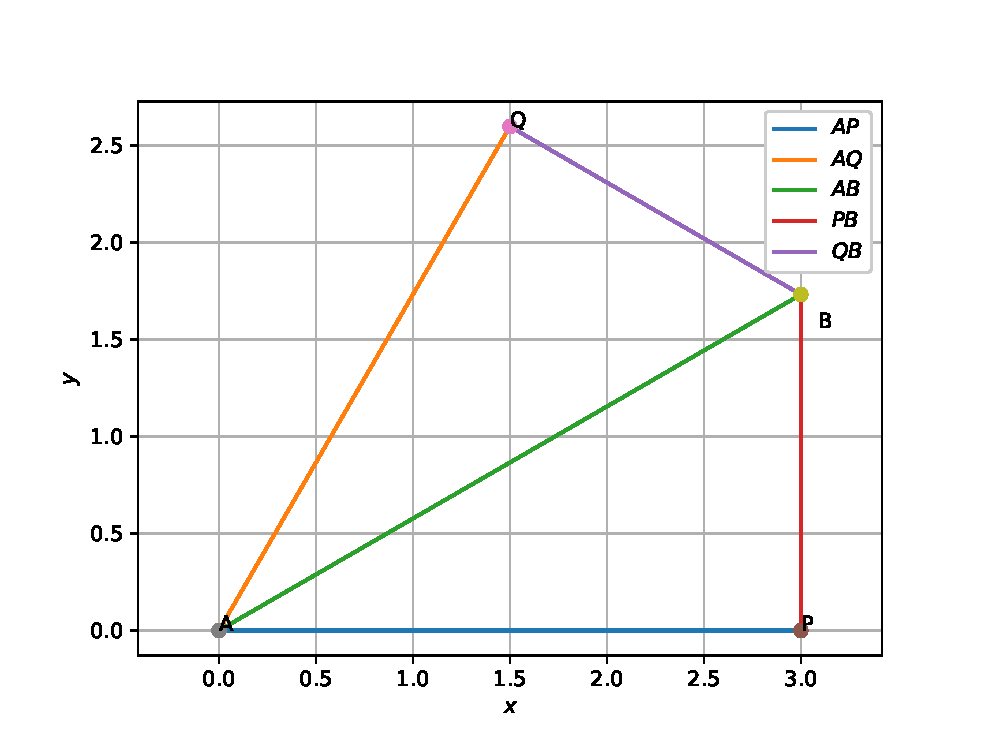
\includegraphics[scale=0.275]{./figs/angle.eps}
\caption{\tiny By Python}
\end{flushleft}

\end{subfigure}
\end{minipage}
\hfill
\begin{minipage}{0.45\linewidth}
\begin{subfigure}{0.4\textwidth}
\begin{flushright}

\resizebox{2.0\columnwidth}{!}{

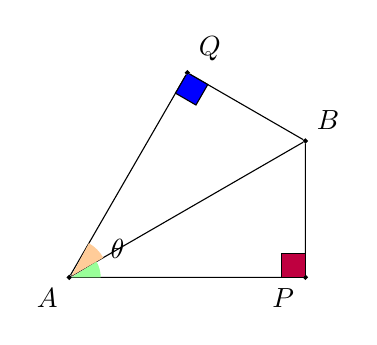
\begin{tikzpicture}
[scale=1,>=stealth,point/.style={draw,circle,fill = black,inner sep=0.5pt},]

\node (A) at (0,0)[point,label=below left:$A$] {};
\node (P) at (3, 0)[point,label=below left:$P$] {};
%\node (Q) at ($({3*\cos{60}}, {3*\sin{60}})$)[point,label=below right:$Q$] {};
%\node (B) at ($({3.4641*\cos{30}}, {3.4641*\sin{30}})$)[point,label=above right:$B$] {};
\node (Q) at (1.5, 2.598)[point,label=above right:$Q$] {};
\node (B) at (3, 1.732)[point,label=above right:$B$] {};




\draw (A) -- node[left] {$\textrm{}$} (P) -- node[below] {$\textrm{}$} (B) -- node[above,xshift=2mm] {$\textrm{}$} (Q);
\draw (A)--(Q);
\draw (A)--(B);


\tkzFillAngle[fill=green!40,size=0.4cm,mark=](P,A,B)
\tkzFillAngle[fill=orange!40,size=0.5cm,mark=](B,A,Q)
\tkzMarkRightAngle[fill=blue,size=.3](A,Q,B);
\tkzMarkRightAngle[fill=purple,size=.3](A,P,B);

%\tkzMarkRightAngle[fill=orange!40,size=0.4cm,mark=](A,Q,B)
%\tkzMarkRightAngle[fill=green!40,size=0.5cm,mark=](A,P,B)

\tkzLabelAngle[pos=0.7](P,A,Q){$\theta$}
%\tkzLabelAngle[pos=0.7](P,A,B){$\gamma$}


\end{tikzpicture}
}
\caption{\tiny By Latex-tikz}
\end{flushright}
\end{subfigure}
\end{minipage}
\end{figure}
\end{frame}


\subsection*{Construction methods}
\begin{frame}[fragile]
\footnotesize
\frametitle{Construction method}
\begin{columns}
\begin{column}{0.5\textwidth}
The tables below are the values used for constructing the triangles in both Python and Latex-Tikz.
\begin{table}[htbp]
\centering
  \resizebox{1\textwidth}{!}{\begin{minipage}{\textwidth}
\begin{tabular}{ |p{2cm}|p{2cm}|  }
\hline
 \multicolumn{2}{|c|}{ Input Values.} \\
\hline
$\vec A$ & $\begin{pmatrix}0\\0\end{pmatrix}$\\
\hline
$\vec P$ & $\begin{pmatrix}3\\0\end{pmatrix}$\\
\hline
$\angle PAQ$ & 60\\
\hline
\end{tabular}
\end{minipage}}
\caption{\tiny To construct $\angle ACB$ and}
\end{table}

\end{column}
\begin{column}{0.5\textwidth}
The steps for constructing $\triangle ACB$ are
\newline
$$\vec{A}= \begin{pmatrix}0\\0\end{pmatrix}
,\vec{P}=\begin{pmatrix}3\\0\end{pmatrix}$$
\\
$$\vec{Q}=\begin{pmatrix}r*\cos{0}\\r*\sin{0}\end{pmatrix}= \begin{pmatrix}3\\0\end{pmatrix}$$
\\
$$\begin{pmatrix}\vec{B} - \vec{P}\end{pmatrix}^T\begin{pmatrix}\vec{A} - \vec{P}\end{pmatrix}= 0$$
$$\angle{\gamma} = \frac{\angle{\theta}}{2} = 30$$
\\


\end{column}
\end{columns}
\end{frame}
\section*{\textbf{}}
\begin{frame}[fragile]
\footnotesize
\begin{columns}
\begin{column}{0.5\textwidth}
	$$\vec{Q}=\begin{pmatrix}b*\cos{\gamma} - 3 \\ b*\sin{\gamma} - 0\end{pmatrix}= \begin{pmatrix}0 - 3\\0 - 0\end{pmatrix}$$
	\\
	$$3*(b*\cos{\gamma} - 3) = 0$$
	\\
	$$b*\cos{\gamma} = 3$$
	\\
	$$b = 3.4641$$
	\\
	$$\vec{B} = \begin{pmatrix}3.4641*\cos{30}\\3.4641*\sin{30}\end{pmatrix} = \begin{pmatrix}3\\1.732\end{pmatrix}$$
	

\end{column}
\begin{column}{0.5\textwidth}
	\begin{table}[H]
		\centering
		\resizebox{0.75\textwidth}{!}{\begin{minipage}{\textwidth}
				\begin{tabular}{ |p{2cm}|p{2cm}|  }
					\hline
					\multicolumn{2}{|c|}{Derived Values for $\angle PAQ$.} \\
					\hline
					$\vec{Q}$ & $$\begin{pmatrix}1.5\\2.59\end{pmatrix}$$\\				
					\hline
					$\vec{P}$ & $$\begin{pmatrix}3\\0\end{pmatrix} $$\\
					\hline
					$\vec{B}$ & $$\begin{pmatrix}3\\1.7\end{pmatrix} $$\\
					\hline
				\end{tabular}
		\end{minipage}}
		\caption{\tiny To construct madians AN and PN}
	\end{table}

\end{column}
\end{columns}
\end{frame}
\subsection{a}
\begin{frame}
\frametitle{Solution a)}
\footnotesize
\label{a}
from the $\Delta APB$ and $\Delta{AQB}$... 
\\
$$\norm{\vec{A-P}} = \norm{\vec{A-P}}$$
\\
$$\angle{AQB} = \angle{APB}$$
\\
$\vec{AB}$ is bisector of $\angle QAP$
\\
$$\implies\angle{AQB} = \angle{APB}$$
\\
thus from ASA conguransy
\\
$$\Delta APB \cong \Delta AQB$$
\end{frame}

\subsection{a}
\begin{frame}
	\frametitle{Solution b)}
$$\Delta APB \cong \Delta AQB$$
\\
$$\implies\norm{\vec{BQ}} = \norm{\vec{BP}}$$

	\centering Hence proved
\end{frame}

\end{document}
